\chapter{Evaluation}

Following the project proposal, evaluation focused on \textbf{expressiveness}, \textbf{correctness} and \textbf{performance}.
As part of expressiveness, I consider Ein's usability as an alternative to NumPy, but also its computational limitations. For the latter criteria, I rely on diverse test and benchmark suites.

\section{Expressiveness}

We evaluate the expressiveness of Ein from two perspectives: \begin{itemize}
    \item For a \textit{programmer}, what patterns are easier to express in Ein than in the established NumPy?
    \item \textit{Computationally}, what can or cannot be expressed in Phi, Ein's formal program representation?
\end{itemize}

\subsection{Programming in Ein}

I argue that Ein is a superior alternative to NumPy-like array frameworks in a variety of cases. 
Ein's design takes advantage of the pointful style and higher-order combinators. 
It introduces language features unseen in the array programming model.
On the other hand, NumPy is occasionally more concise and is much more mature as software, but often generalises badly to non-standard operations. 
To illustrate the key points, we follow a few case studies and discuss the differences between Ein and NumPy implementations.

\subsubsection{Logits in a Graph Attention Network}

Our flagship example of an unwieldy many-dimensional operation is the logit computation in a Graph Attention Network (GAT), as introduced in the very first chapter. The NumPy implementation below was paraphrased from the original real-world Jax code (the interface of which is based on NumPy):
\begin{center}
\begin{cminted}{python}
def logits(att_1, att_2, att_e, att_g):
    return (
        transpose(expand_dims(att_1, axis=-1), (0, 2, 1, 3)) +  # + [B, H, N, 1]
        transpose(expand_dims(att_2, axis=-1), (0, 2, 3, 1)) +  # + [B, H, 1, N]
        transpose(att_e, (0, 3, 1, 2)) +                        # + [B, H, N, N]
        expand_dims(expand_dims(att_g, axis=-1), axis=-1)       # + [B, H, 1, 1]
    )                                                           # = [B, H, N, N]
\end{cminted}
\end{center}
We re-express this in the following Ein code:
\begin{center}
\begin{cminted}{python}
def batch_logits(s, t, e, g):
    return array(lambda h, u, v: s[u, h] + t[v, h] + e[u, v, h] + g[h])

def logits(att_1, att_2, att_e, att_g):
    return array(lambda b: batch_logits(att_1[b], att_2[b], att_e[b], att_g[b]))
\end{cminted}
\end{center}
It is worth remarking that the Ein code compiles into NumPy calls which are just as efficient as the base implementation. We move on to discuss the key differences:

\begin{description}
    \item[Shape manipulation] The array programming model revolves around manipulating array shapes to `align' them for subsequent whole-array operations. This does not generalise well to \textbf{many-dimensional data} -- the code becomes polluted with \textit{axis indexing}. The syntax of the applied operations is unhelpful in determining their semantics. In contrast, Ein code relies on index-oriented descriptions. Extending the implementation with another dimension is just adding another index -- rather than modifying fragile arguments to routines (like in NumPy). Additionally, index names serve to hint at the meaning of array dimensions -- like variable names hint at data they store.
    % this is reminiscent of manipulating a program in a de Bruijin index representation, which is not convenient for a human.  
    \item[Batching] The Ein code is different from what was foreshadowed in the Introduction. We separated out \textcolor{blue}{\texttt{batch\_logits}}, which does most of the work, but disregarding the \textit{batch axis} (named \texttt{b}). A batch axis is a pervasive code structuring technique in NumPy code, which allows mapping an operation over many inputs (for the \texttt{att\_*} arrays it is denoted \texttt{B} in comments). It is assumed that it will be carried through in broadcasting. In Ein, we instead settle for a functional-esque approach, and explicitly map elements across each index \texttt{b}. This is clearer in intent and avoids arbitrary code conventions.
\end{description}

\subsubsection{Min-plus matrix multiplication}

We now consider the case of min-plus (or \textit{tropical}) matrix multiplication, which is relevant in shortest path problems. For a pair of matrices $A$ and $B$, its result is a matrix $D$ given by $D_{i,j} = \min_{k} A_{i,k} + B_{k,j}$ (like a usual matrix product, but in a $(\min, +)$ semiring instead of $(+, \times)$). We compare equivalently efficient NumPy and Ein implementations that compute this product in $\mathcal O(n^2)$ space.

\begin{center}    
\begin{minipage}[t]{.5\textwidth}
\raggedright
\begin{center}    
\begin{cminted}{python}
def min_plus_product(a, b):
    n,  m = a.shape
    m_, k = b.shape  # m == m_
    d = full((n, k), float("+inf"))
    for t in range(m):
      d = minimum(
        d, 
        expand_dims(a[:, t], axis=1) + b[t, :]
      )
    return d
\end{cminted}
\end{center}
\end{minipage}%
\begin{minipage}[t]{.5\textwidth}
\raggedleft
\begin{center}    
\begin{cminted}{python}

def min_plus_product(a, b):
    return array(
      lambda i, j: fold(
        float("+inf"),
        lambda k, acc: min(
            acc, 
            a[i, k] + b[k, j]
    )))

\end{cminted}
\end{center}
\end{minipage}
\end{center}

\begin{description}
    \item[Reasoning about shape] In this example, it is necessary to directly access NumPy array shapes to initialise the accumulator and compute the number of iterations. Code clarity requires introducing additional variables \texttt{n, m, k} to the code, disconnecting them from \texttt{a} and \texttt{b} which they describe. In Ein, \textbf{size inference} is sufficient to assign the right sizes and iteration counts in common cases.
    \item[Data-parallel loops] A space-efficient NumPy implementation necessitates a loop with a matrix accumulator. 
    % Using broadcasting instead would be more convenient, but would use excessive amounts of memory due to an intermediate cubic-size array. 
    Data-parallel loops like this are simple to express with Ein's \texttt{fold}. We avoid point-free reasoning about a matrix accumulator, instead focusing on a fixed index \texttt{(i, j)}.
    Arguably, the \texttt{fold} syntax is far from ideal, but readability could be helped with a shorthand:
    \begin{center}        
    \begin{cminted}{python}
def fold_min(f):
    return fold(float("+inf"), lambda k, acc: min(acc, f(k)))
d = array(lambda i, j: fold_min(lambda k: a[i, k] + b[k, j]))
    \end{cminted}
    \end{center}
\end{description}

\subsubsection{Pairwise $L_1$ distances}

The last example computes the sum of absolute differences ($L_1$ distance) between every pair of rows of a matrix \texttt{A}. 
% This operation has the following index-oriented specification:
% $$ \texttt{pairwiseL1(A)}_{i,j} = L_1(\texttt{A}_i, \texttt{A}_j) = \sum_k \left| \texttt{A}_{i,k} - \texttt{A}_{j,k} \right| $$
We compare NumPy (as in \cite{maclaurin2019dex}) and Ein implementations:
\begin{center}    
\begin{minipage}[t]{.5\textwidth}
\raggedright
\begin{center}    
  \begin{cminted}{python}
def pairwiseL1(A: ndarray) -> ndarray:
  return sum(
    abs(transpose(A, (1, 0)) 
        - expand_dims(A, axis=2)),
    axis=1)
  \end{cminted}
\end{center}
\end{minipage}%
\begin{minipage}[t]{.5\textwidth}
\raggedleft
\begin{center}    
  \begin{cminted}{python}
def L1(u: Vec[Float], v: Vec[Float]) -> Float:
  return reduce_sum(lambda i: abs(u[i] - v[i]))

def pairwiseL1(A: Vec[Vec[Float]]):
  return array(lambda i, j: L1(A[i], A[j]))
  \end{cminted}
\end{center}
\end{minipage}
\end{center}
\begin{description}
    \item[Separation of concerns] The Ein implementation separates the computation of $L_1$ distances into the function \textcolor{blue}{\texttt{L1}} -- this is difficult to replicate in NumPy. By forcing reasoning on whole arrays, the array programming model actively discourages encapsulation. For example, say we want to generalise the code to different distances. A higher-order NumPy \textcolor{blue}{\texttt{pairwiseL1}} parameterised by the distance function would necessitate a certain contract (like with the batch axis convention). In contrast, Ein's \textcolor{blue}{\texttt{pairwiseL1}} could be rewritten to take any distance function \texttt{dist} of the same signature as \textcolor{blue}{\texttt{L1}}:
    \begin{center}
    \begin{cminted}{python}
def pairwiseL1(A: Vec[Vec[Float]], dist: (Vec[Float], Vec[Float]) -> Float):
    return array(lambda i, j: dist(A[i], A[j]))
    \end{cminted}
    \end{center}
    \item[Type signatures] NumPy's support for type signatures is poor. Type checking by standard tools like \texttt{mypy} is even more problematic, and only partially solved by bespoke extensions \cite{liu2020type}. In contrast, Ein's type system is simple and behaves well under composition. Ein code can have useful static type checking performed by \texttt{mypy}. Furthermore, \texttt{mypy} can infer the return type of \textcolor{blue}{\texttt{pairwiseL1}} -- \texttt{Vec[Vec[Float]]}. This is a stark difference to the failings of typing NumPy programs.
\end{description}
% In addition, points we discussed prior hold just as strongly in this case -- Ein code is much clearer than the NumPy equivalent, necessitating no fragile code (e.g. from the use of axis indexing).

% \paragraph{Functions}
% \paragraph{No rank polymorphism}

\subsection{Computation in Phi}

Having considered the practicalities of Ein, we consider its computational limitations on the basis of Phi. We refer to known theory and features present in other array languages.

\paragraph{Primitive recursion} 
Phi is not Turing-complete -- all programs terminate. 
A lower bound on its expressive power is given by primitive recursive functions. 
Indeed, $\mathrm{fold}$ directly corresponds to primitive recursion $\rho$. 
Nevertheless, we argue Turing-complete computations are seldom necessary in array programming -- for instance, no native NumPy routines involve unbounded search. 
Since Ein is an embedded DSL, we can rely on the generality of its host language, Python -- this is standard practice. 
% We further lack control flow primitives like conditional branches, a design choice for which we argued in the Implementation chapter -- Phi's limitations seek to meet in the middle with what is efficient in hardware.

\paragraph{Lack of in-place updates} A major limitation of Phi is the lack of support for in-place updates (in particular, at an array index like in \mintinline{c}{a[5] = 42}). 
This leads to higher computational complexity in some cases. 
Since Ein is purely functional, we cannot simply rely on side effects to handle updates.
To this end, Futhark uses a uniqueness type system, while Dex makes use of an effect system \cite{henriksen2017futhark, paszke2021getting}. 

It is worth noting in-place updates can be (unsafely) replicated through the use of extrinsics as follows: 
\begin{center}    
\begin{cminted}{python}
def update(vec: Vec[Scalar], p: Scalar, x: Scalar) -> Vec[Scalar]:
    def with_update(arr: ndarray, pos: int, val: int) -> ndarray:
        arr[..., pos] = val; return arr
    return ext(with_update, vec.expr.type)(vec, p, x)    
\end{cminted}
\end{center}
Here, \texttt{update} mutates its \texttt{vec} argument, returning \mintinline{python}{array(lambda i: where(i != p, vec[i], x))}. Careless use leads to unexpected behaviour, but the approach exemplifies how extrinsics can be used to extend Ein.


\paragraph{Parallelism} Ein offers only limited support for common computational patterns. Though associative reductions were implemented as an extension, there are many other examples of useful parallel programming patterns. These are best exemplified by Futhark's array combinators -- particularly scan, histograms (\textit{scatter} in the context of GPU programming), and filtering. Only some can be efficiently interpreted by calling out to NumPy routines, pointing to possible extensions to its interface.

\section{Correctness}

Formally proving the correctness of compilers is difficult \cite{kumar2014cakeml}. 
I settled for a robust test suite testing runtime correctness.

\subsection{Tests}

Ein's test suite (implemented in the \texttt{pytest} framework) mainly consist of compiled program output correctness in a variety of settings. 
I distinguish three kinds of such tests:
\begin{itemize}
    \item 13 Phi/IR-level tests. These consist of small program definitions directly in the Phi calculus. They are essentially unit tests for the na\"ive Phi interpreter.
    \item 59 Ein tests of small to medium length, which are implemented through Ein's API. This includes feature-specific tests for: extrinsics (4 tests), records (7 tests), and the PyTorch backend (6 tests).
    \item 9 \textit{case} tests, which are longer. They were constructed from publicly open array programs. We also use these for benchmarking (see Section \ref{benchmarks}).
\end{itemize}

Correct outputs are generated with Python reference code.
To obtain baseline outputs for Phi programs constructed by Ein I use the na\"ive Phi interpreter.
This allows diagnosis whether the problem is with the compiler to Yarr or the source Phi.
Outputs are treated as correct even when equality is approximate, as many tests use floating point arithmetic. 
Specifics of floating point semantics are often disregarded in domains like machine learning due to the limitations they cause in optimisations -- for instance, famously floating point addition is not associative \cite{alawi2004every}.

Most tests are parameterised by execution backend (through \texttt{pytest.mark.parametrise}) and run on random inputs. Since control flow in Phi is limited, random data is essentially sufficient to capture whether compiled programs behave correctly. 

The entire test suite passes successfully. The test line coverage across the implementation was measured to be \textbf{92\%}. Most of the untested code is in error paths, which were tested less often. Tests instead focus on ensuring that correct Ein/Phi programs behave correctly. Checking that bad programs fail gracefully would mostly serve to test user experience, which was not part of the success criteria.

\subsection{Defensive programming}

To improve the capability of tests to pick up bad behaviour in internal parts of the implementation, a form of \textit{defensive programming} was applied throughout project code.
This was only a general practice of ensuring expected compiler invariants are met through Python \mintinline{python}{assert} statements. Failing an assertion generally indicates an internal compiler error and hence a bug. 

\needspace{2em}
We consider a few examples of this defensive approach: \begin{itemize}
    \item Types in the array-of-structs to struct-of-arrays program transformation are mapped in a consistent way ($\phisoa{\phivectype{(\phipairtype{\tau_1}{\tau_2}})} = \phipairtype{\phivectype{\tau_1}}{\phivectype{\tau_2}}$). We assert this mapping is upheld for each subexpression.
    \item Outlining asserts the original program $p$ and $\mathrm{inline}(\mathrm{outline}(p))$ are equal. Therefore, we ensure let-bindings inserted preserve program semantics.
    \item We check that all Phi and Yarr terms constructed within the compiler are well-typed.
\end{itemize}
% By testing invariants through program assertions and including feature-specific tests, a diverse component testing suite is formed. 

\section{Performance}

Ein's code-generation phase results in a Yarr program, which is by default interpreted by calling respective NumPy routines. 
Hence, our choice of compilation target (and runtime) is unique in the regard it is rather high-level.
The `machine instructions' are NumPy routines, and hence the we are limited by its performance characteristics. 
Generally it is sensible to compare compiler-generated programs against a baseline.
We form a suite of baseline NumPy programs and compare Ein's performance on a varied suite of benchmarks.

\subsection{Benchmarks}
\label{benchmarks}

We benchmark array programs generated by Ein against baseline NumPy implementations.
However, the choice of baselines is inherently subjective -- for any Ein-generated program using NumPy, there is a just as fast program using NumPy directly.
For a fair comparison, I aimed for \textit{idiomatic} NumPy code without particular optimisations applied.
We consider Ein to be efficient if at large problem sizes the running time is within a small constant factor of the baseline. 


\begin{table}[b]
    \centering
    \begin{tabular}{c|c|l}
       \textbf{Benchmark} & \textbf{Source} & \textbf{Description} \\ \hline
        Attention & Open-source & core part of Neural Attention \\
        GAT & Open-source & inference in the Graph Attention Network architecture \\
        Semirings & Based on \textcite{dolan2013fun} & shortest paths via closure of a tropical semiring matrix \\
        MRI-Q & Parboil & basic linear reduction \\
        Stencil & Parboil & basic 3D stencil \\
        Hotspot & Rodinia & complex 2D stencil \\
        Pathfinder & Rodinia & 1D dynamic programming 
    \end{tabular}
    \caption{Brief overview of each of the Ein benchmark cases. They are also included in the test suite as system tests.}
    \label{tab:benchmarks}
\end{table}


\paragraph{Suite} Our benchmark suite (\ref{tab:benchmarks}) builds on the findings from Section \ref{suite-review}. We mainly base on cases implemented in the Futhark benchmarks \cite{The_Futhark_Hackers_futhark-benchmarks} (as done by Dex), as well as open-source implementations of deep learning architectures.
I hand-translated all of the cases from the source language (Futhark, or Python using PyTorch/Jax) into equivalent a pair of programs in Python using Ein or NumPy.

A benchmark case worth special note is \textit{Semirings}, which was implemented from scratch. 
The NumPy baseline is a standard $\mathcal O(n^3)$ implementation of the Floyd-Warshall all-pairs shortest paths algorithm. 
In Ein, I instead make rich use of arrays of user-defined dataclass types. 
I follow the approach of \textcite{dolan2013fun} for solving a general family of problems via matrices over a \textit{closed semiring}%
\footnote{A \textit{semiring} is an algebraic structure $(+, \times)$, where the operation $+$ is a `choice' and $\times$ a `sequencing', with identity elements $0$ and $1$. \textit{Closed semirings} further define an operation $a^*$ which computes $a^* = 1 + a + a^2 + \cdots$. These structures necessarily follow certain algebraic laws. The \textit{tropical semiring} turns out to capture the computation of shortest paths in a graph.}.
We implement his generic approach in Ein, taking advantage of efficient array operations.
% By implementing the \texttt{Tropical} instance of a \texttt{Semiring}, we can compute the closure of a generic \texttt{SemiringMatrix}, yielding the shortest paths.
NumPy lacks similarly capable abstractions, and in Ein we show they are of zero cost.
See Figure \ref{fig:semirings} for the crux of the generic Ein implementation.

\begin{figure}
    \centering
\begin{cminted}{python}
class SemiringMatrix:
    ...
    def closure(self):
        return SemiringMatrix(fold(
            self.elem,
            lambda k, acc: array2(
                lambda i, j: acc[i, j] + acc[i, k] * acc[k, k].closure() * acc[k, j]
        ).assume(self.elem[k, k]))) + self.one
\end{cminted}
    \caption{Closure of a \texttt{SemiringMatrix} in Ein (Algorithm 6.1 \cite{abdali1985transitive}). \texttt{+}, \texttt{*} are overloaded \texttt{Semiring} operations. When \texttt{+} is $\min$ and \texttt{*} is $+$, this reduces to the Floyd-Warshall shortest paths algorithm.}
    \label{fig:semirings}
\end{figure}

It is worth note that the other two cases used in the test suite -- NN and KMeans (from Rodinia) -- were excluded from the benchmark. A computationally efficient implementation of these relies on features unavailable in Ein (respectively in-place updates and histogram computations). They could be mimicked through extrinsics in practice, but their use would not constitute a useful benchmark.

\paragraph{Methodology} Benchmarks were conducted on a M1 Pro MacBook (14-inch, 2021). The versions used were Python \texttt{3.11.6} and NumPy \texttt{1.26.4}. No further thread parallelism was used beyond what is used by default in NumPy (in linear algebra routines). Large problem sizes are used (about 1 second of execution time), taking the minimum time across at least 5 runs. 

\begin{figure}[b]
    \centering

    \pgfplotsset{
    /pgfplots/baseline legend/.style={
    legend image code/.code={
    \draw[thick,draw,color=red](-0.05cm,0cm) -- (0.3cm,0cm);%
       }
      }
    }
    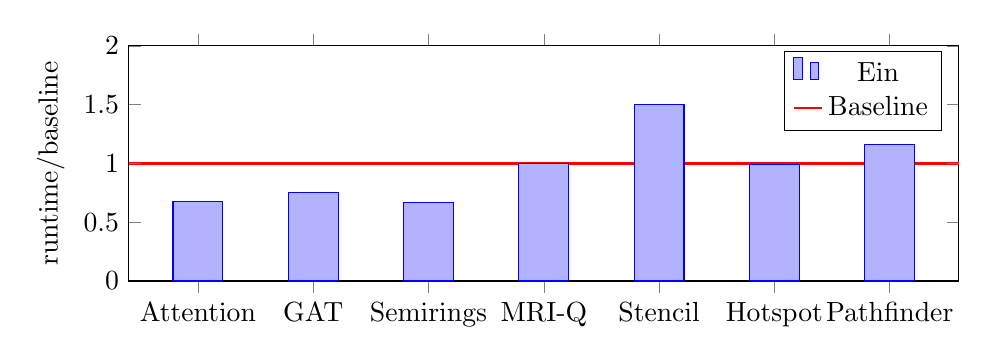
\begin{tikzpicture}
        \begin{axis}[
            ybar,
            ymin=0,
            ymax=2,
            extra y ticks = 1,
            extra y tick labels={},
            extra y tick style={grid=major,major grid style={thick,draw=red}},
            symbolic x coords={Attention, GAT, Semirings, MRI-Q, Stencil, Hotspot, Pathfinder},
            legend entries={Ein, Baseline},
            xtick=data,
            ylabel={runtime/baseline},
            bar width=1.8em,
            width=\linewidth,
            height=13em,
        ]
    
        \addplot[draw=blue, fill=blue!30] coordinates {
            (Attention, 0.68) 
            (GAT, 0.75) 
            (Semirings, 0.67)
            (MRI-Q, 1.0) 
            (Stencil, 1.5)
            (Hotspot, 0.99)
            (Pathfinder, 1.16)
        };
        \addlegendentry{Ein}
        \addlegendimage{baseline legend}
        \addlegendentry{Baseline}
    
        \legend{Ein, Baseline}
        
        \end{axis}
    \end{tikzpicture}

    \caption{Ratio of the running time of Ein-generated NumPy programs, and the baseline NumPy. \textit{Lower is better.}}
    \label{fig:benchmark-results}
\end{figure}


\paragraph{Discussion} Benchmark results can be seen in Figure \ref{fig:benchmark-results}. Results are generally promising -- Ein is no more than 60\% slower, and in some cases it is 40\% faster. 
Generally, where Ein outperforms the baseline, it is thanks to operating in-place to avoid allocation of temporaries. 
Performance deficits are especially due to missing advanced indexing strategies -- particularly in Stencil. 
However, the downside of the baseline's performance on Stencil is the inclusion of error-prone expressions like \mintinline{python}{A[1:-1, :-2, 1:-1]} (some 10 times).
We conclude Ein offers a good trade-off on code readability and performance.

\newpage
\section{Work completed}

We overview the work completed basing on the success criteria from the proposal: \begin{description}
    \item[Embedding an array language in Python] The implemented \texttt{ein} library successfully embeds\footnote{The original proposal unfortunately contained a misunderstanding of the phrase \textit{shallow} embedding. In reality, the intended meaning was that of a \textit{deep} embedding. This mistake was corrected after further literature search.} a pointful array language -- Ein -- in Python. Ein's API builds up terms in the Phi calculus, after which it allows calling out to the compiler to evaluate the program with an execution backend. Key extensions on the proposed core interface are: size inference, general \texttt{fold} and \texttt{reduce} combinators, extrinsics, rich record types, support for type annotations.
    \item[Designing a pointful array calculus] Phi was designed successfully, and ended up building on the $\tilde F$ language due to \textcite{shaikhha2019efficient}. This further includes various extensions with respect to the proposal: fully-fledged pair types, size assertions, folds, and associative reductions.
    \item[Efficient execution backend] We compile pointful array programs (in the Phi calculus) by generating point-free array code (Yarr calculus) using the mathematical foundation of Axials. Yarr programs can be efficiently interpreted by calling NumPy routines. A key extension was the inclusion of a PyTorch backend, taking advantage of hardware acceleration and automatic differentation.
\end{description}
Ein's compiler middle-end was also suitable for extensions: the array-of-structs to struct-of-arrays transformation and outlining (common subexpression elimination and loop-invariant code motion).

\section{Summary}

Throughout this chapter we have seen that Ein is expressive, and can be superior in usability as an alternative to NumPy. 
It further has various language features unseen in NumPy-like frameworks.
Furthermore, robust tests ensure correctness of our implementation. 
Benchmarking has shown our execution backend is efficient on a varied suite of cases. 
Ein leads to much clearer programs than what would be written by a NumPy programmer, while preserving -- or even improving -- performance. 
